\documentclass[11pt]{article}
                                      
\usepackage{fullpage}					% full page dimensions
%\usepackage[letterpaper,hmargin=1in,vmargin=1in]{geometry}

\usepackage{amsmath}                    % special AMS math symbols
\usepackage{amssymb}                    % special AMS math symbols
\usepackage{color}                      % colored text and backgrounds

\usepackage{indentfirst}
\usepackage{framed}

\usepackage{algorithm} 
\usepackage{algpseudocode}

\usepackage{verbatim}

\usepackage{graphicx}                   % graphics
\usepackage[caption=false, font=footnotesize]{subfig}
%\usepackage{tabularx}

%\usepackage{epstopdf}
%\usepackage{amsthm}
%\usepackage{multirow}

%\usepackage{subcaption}
%\usepackage{comment}
%\usepackage{framed}
%\usepackage{hyperref}


\begin{document}

\title{Anonymous DTN routing}
\maketitle

%%%%%%%%%%%%%%%%%%%%%%%%%%%%%%%%%%%%%%%%%%%%%%%%%%%%%%%%%%%%%%%%%%%%%%%%%%
\section{Experimental Result}
%%%%%%%%%%%%%%%%%%%%%%%%%%%%%%%%%%%%%%%%%%%%%%%%%%%%%%%%%%%%%%%%%%%%%%%%%%
\subsection{Overview}

\subsubsection{Simulation model}
\begin{itemize}
 \item ONE simulator, default scenario/setting

 \item Map: Helsinki (4500m * 3500m)

 \item Nodes: 246 (160 humans, 80 cars, 6 trams)
  \begin{itemize}
   \item Packet buffer: Humans and cars (50MB), trams (500MB).
   \item Contact interval: Humans (2 mins 30 secs), cars (1 min), trams ( 40 secs)
  \end{itemize}

 \item Packet(message) generation
  \begin{itemize}
   \item Packet size: 500KB - 1MB
   \item Packet generation interval: 35sec - 50sec
   \item TTL: 5 hours
  \end{itemize}

 \item Movement: Random way point, map-based movement.

 \item Network interface: bluetooth, wlan (determine communication distance and bandwidth)
  \begin{itemize}
   \item Humans, cars: Bluetooth (Bandwidth: 2Mbps, Communication range: 10m)
   \item Trams: WLAN (Bandwidth: 10Mbps, Communication range: 100m)
  \end{itemize}

 \item Simulation running time: 12 hours
\end{itemize}



\subsubsection{Anonymous DTN routing setup}
\begin{itemize}
 \item \# group: 1
 \item \# nodes in a group: varies from 5\% to 30\%
 \item Epoch: varies from 10 mins to 60 mins
 \item Base routing protocol: epidemic (flooding)
\end{itemize}



\subsubsection{Assumptions \& simplification}
\begin{itemize}
 \item Communication within a group\\
Only nodes belong to any ``group'' can send packets to other nodes it trusts. 
Nodes that don't belong to any group cannot generate packets.

 \item Strict time sync\\
Epoch starts exactly at the same time in all nodes

 \item No ``beacon'', ``hello'', ``pull'' messages\\
Once two nodes are located within a specific distance, they know ephemeral addresses, packet digest, pulling list of each other without any message exchange. 

 \item Forwarding policy\\
On contact, a node first forwards packets whose destinations are either trusted by the next-hop node or in neighbor list of the next-hop node.  Then it tries to forward remaining packets in FIFO manner. 
\end{itemize}


\subsection{Results}






% delivery rate
\begin{figure}[h!]
\center
\subfloat[Delivery rate: Ephemeral ID valid for 3 epochs]{%
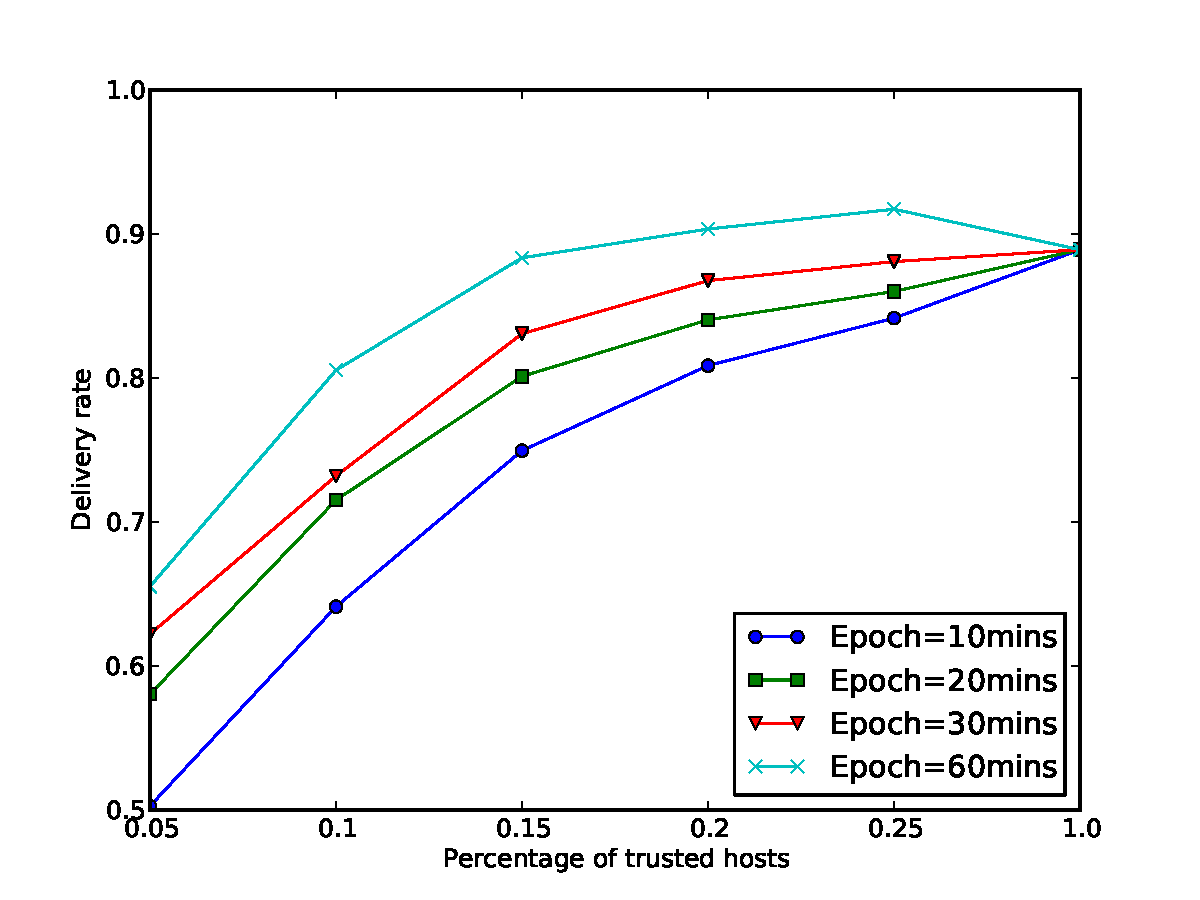
\includegraphics[width=0.49\columnwidth]{figures/epoch_3/delivery_rate.pdf}
\label{fig:delivery_rate_3}
}
\hfill
\subfloat[Delivery rate: Ephemeral ID valid for 6 epochs]{%
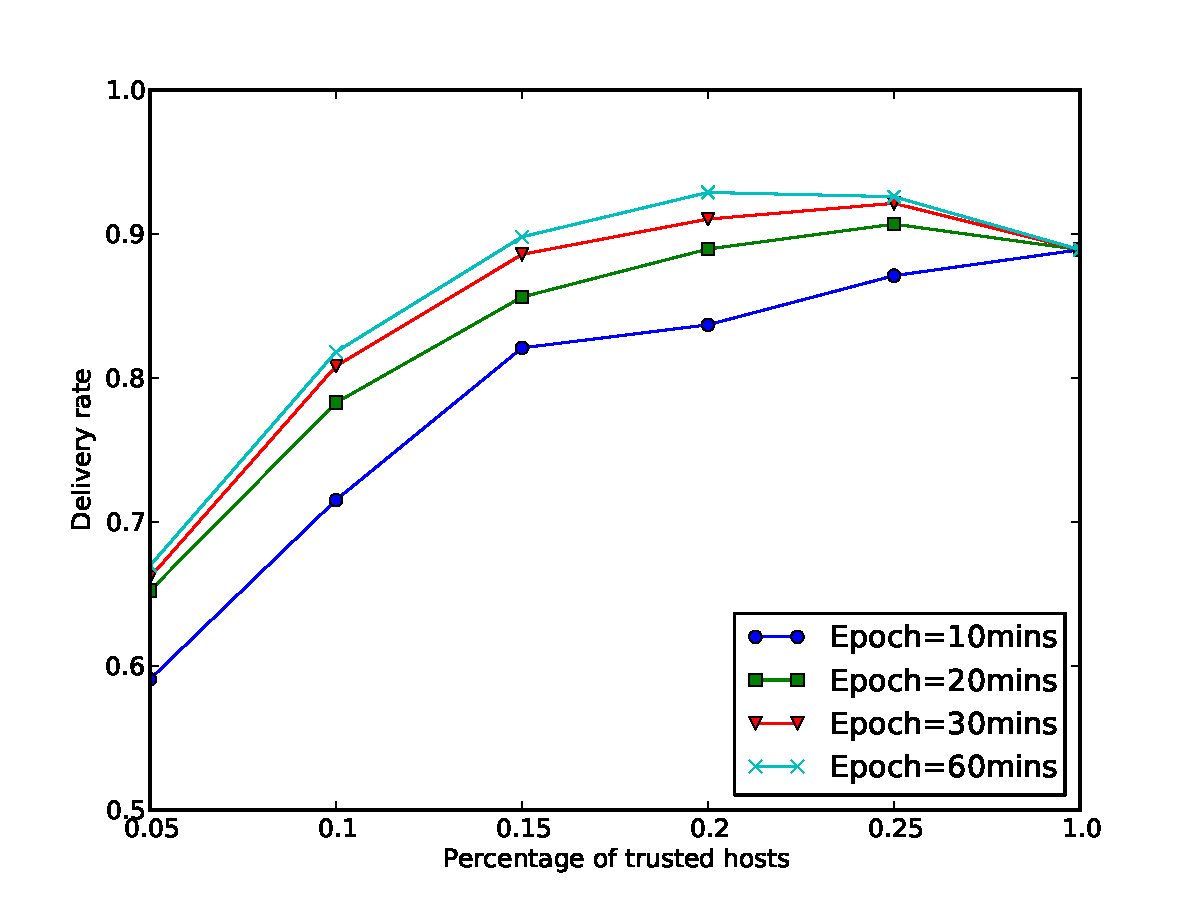
\includegraphics[width=0.49\columnwidth]{figures/epoch_6/delivery_rate.pdf}
\label{fig:delivery_rate_6}
}
\caption{{\bf Packet delivery rate.} 
Delivery rate of pure epidemic routing protocol: 75.88\%. 
Increasing ephemeral ID duration from 3 epochs to 6 epochs enhances the delivery rate slightly, but not significantly.
}
\label{fig:delivery_rate}
\end{figure}


% hop count
\begin{figure}[h!]
\center
\subfloat[Delivery hop count: Ephemeral ID valid for 3 epochs]{%
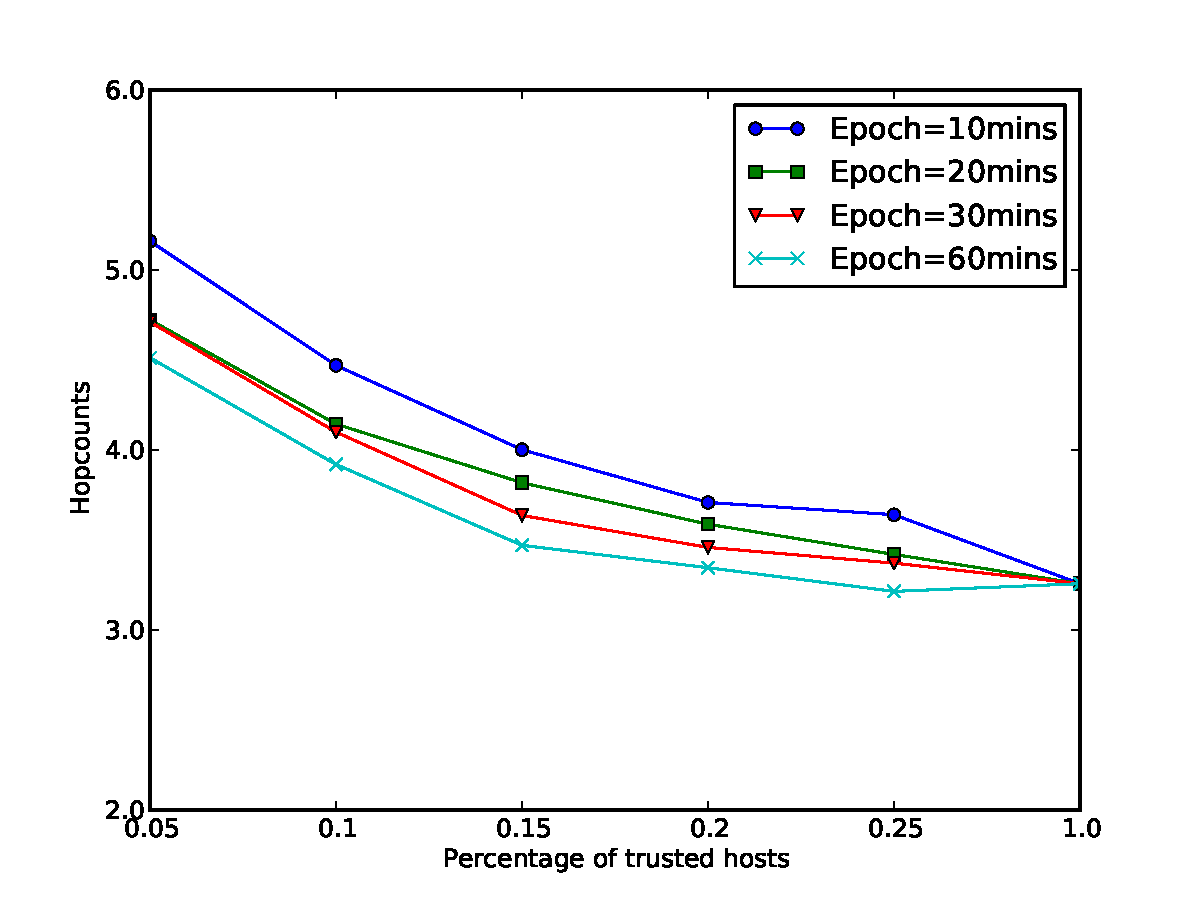
\includegraphics[width=0.49\columnwidth]{figures/epoch_3/hopcount.pdf}
\label{fig:delivery_hopcount_3}
}
\hfill
\subfloat[Delivery hop count: Ephemeral ID valid for 6 epochs]{%
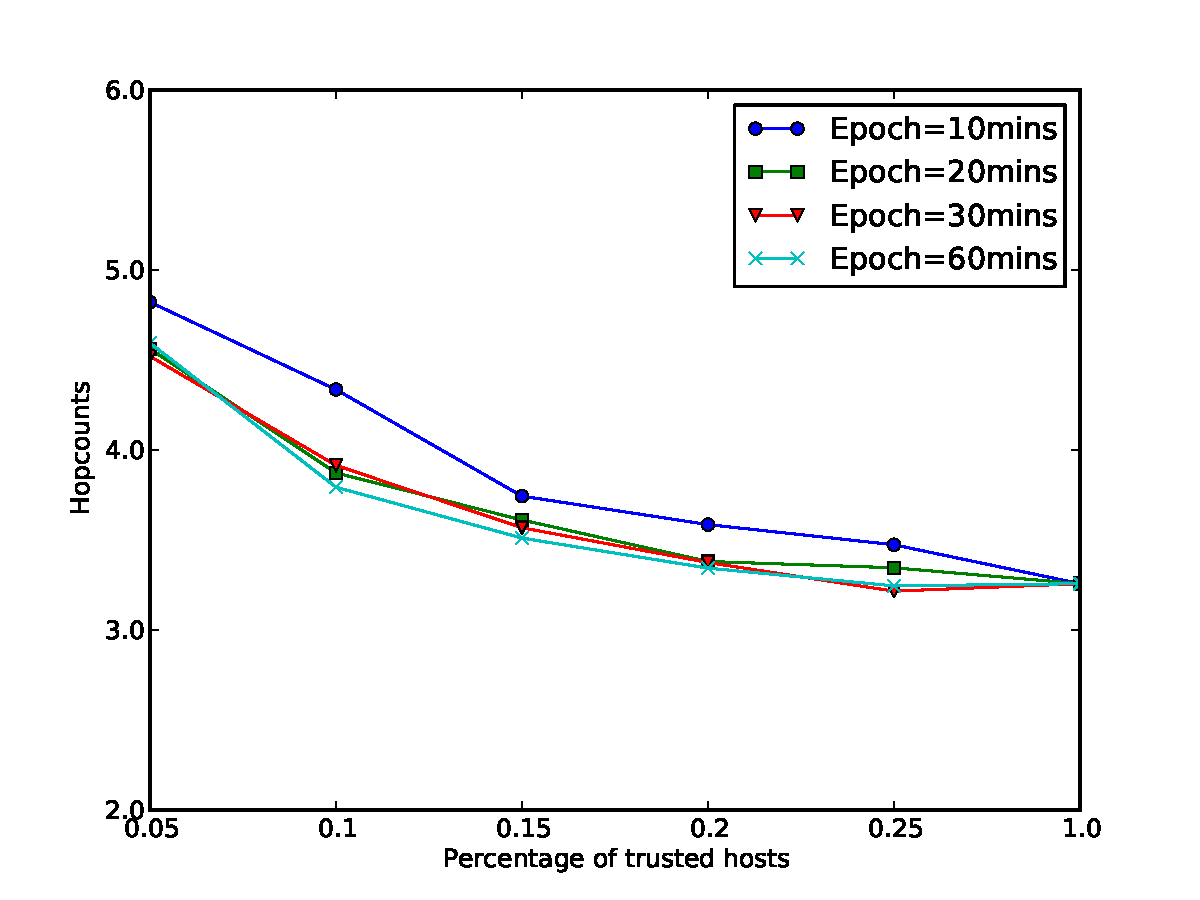
\includegraphics[width=0.49\columnwidth]{figures/epoch_6/hopcount.pdf}
\label{fig:delivery_hopcount_6}
}
\caption{{\bf Packet delivery hop count.}
Delivery hop count in Figure~\ref{fig:delivery_hopcount_3} and \ref{fig:delivery_hopcount_6} are higher than that of pure epidemic routing, especially when the percentage of trusted nodes is low due to inefficient routing using small number of trusted nodes.
}
\label{fig:delivery_hopcount}
\end{figure}



% delivery latency
\begin{figure}[h!]
\center
\subfloat[Delivery latency: Ephemeral ID valid for 3 epoch]{%
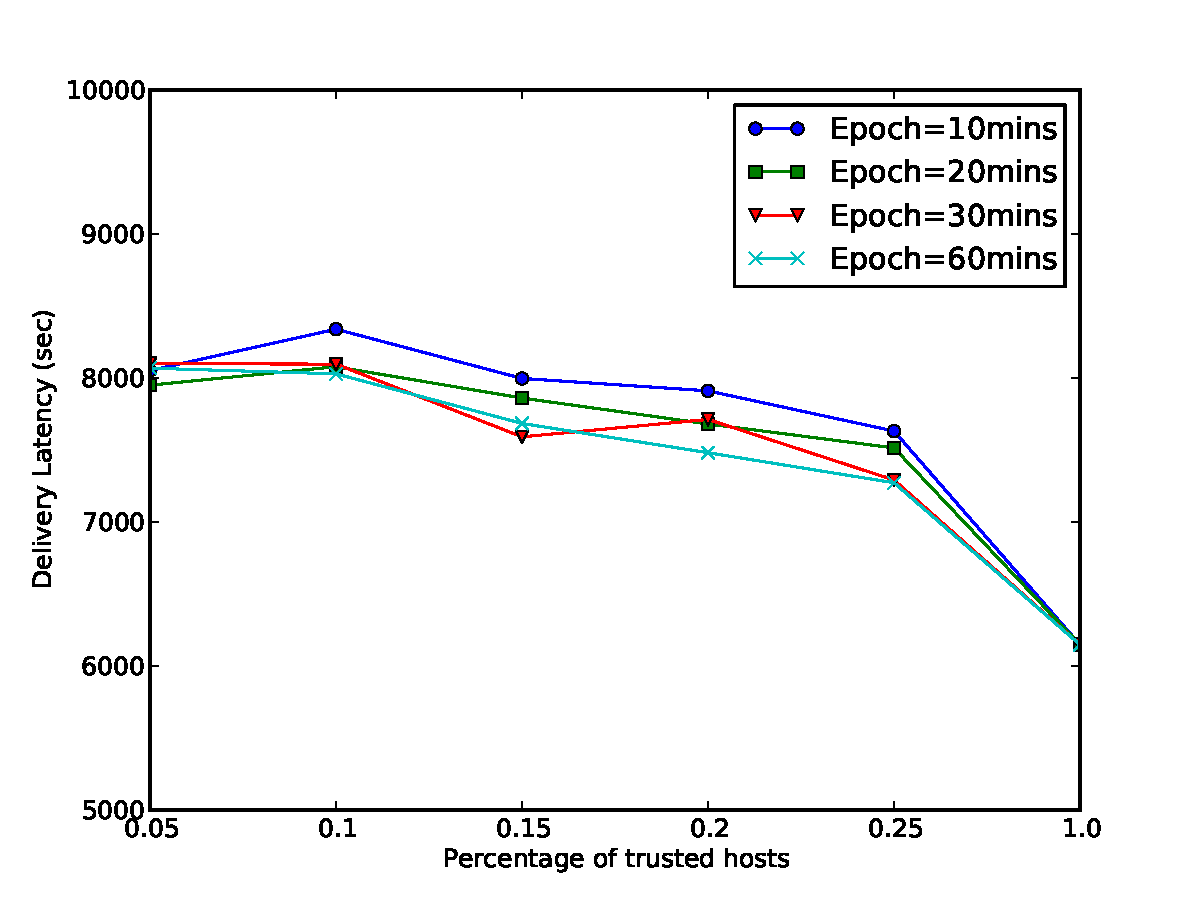
\includegraphics[width=0.49\columnwidth]{figures/epoch_3/delivery_latency.pdf}
\label{fig:delivery_latency_3}
}
\hfill
\subfloat[Delivery latency: Ephemeral ID valid for 6 epochs]{%
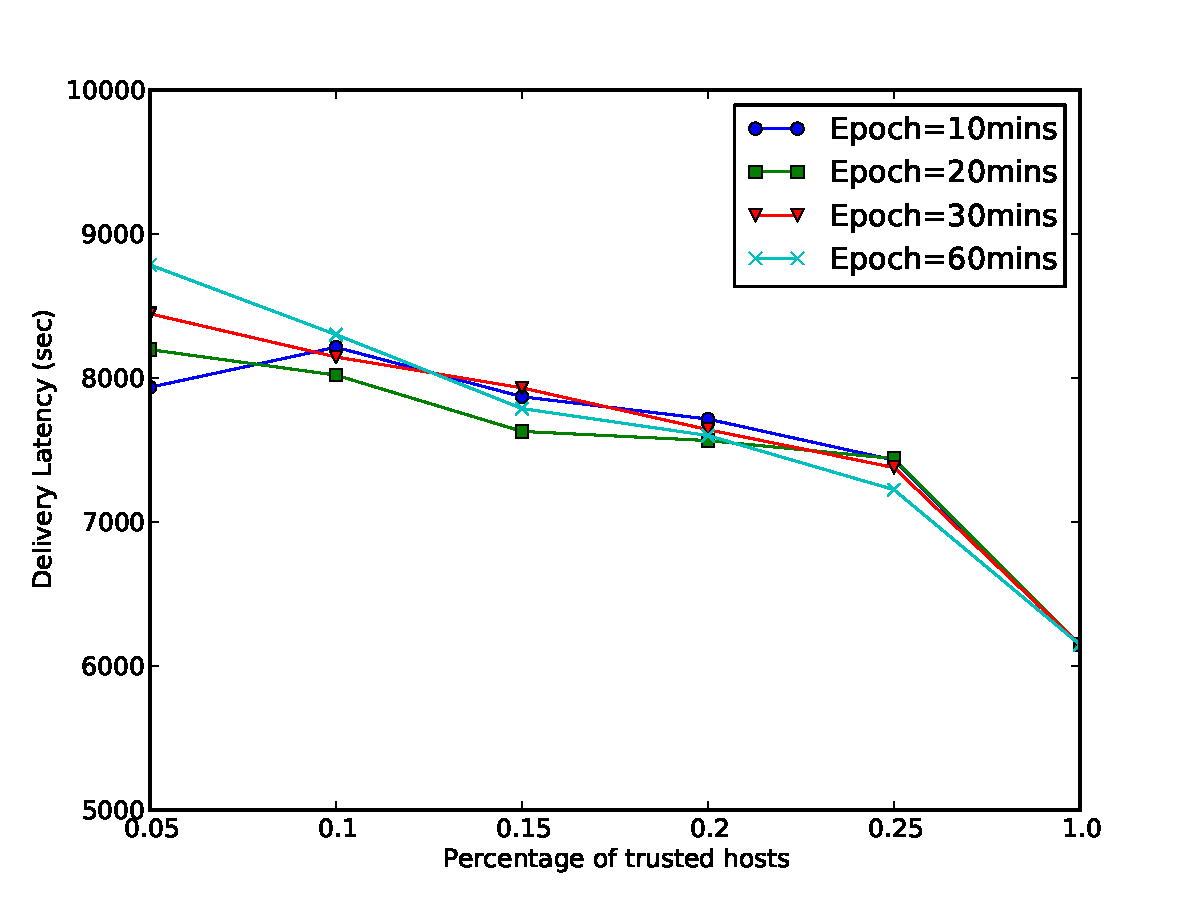
\includegraphics[width=0.49\columnwidth]{figures/epoch_6/delivery_latency.pdf}
\label{fig:delivery_latency_6}
}
\caption{{\bf Packet delivery latency.}
Packet delivery latency in Figure~\ref{fig:delivery_latency_6} is little bit higher than that in Figure~\ref{fig:delivery_latency_3}, probably because of higher delivery rate.
}
\label{fig:delivery_latency}
\end{figure}








% overall packet relay count / delivered packet relay count 
\begin{figure}[h!]
\center
\subfloat[Relay count of overall packets. Ephemeral ID valid for 3 epochs.]{%
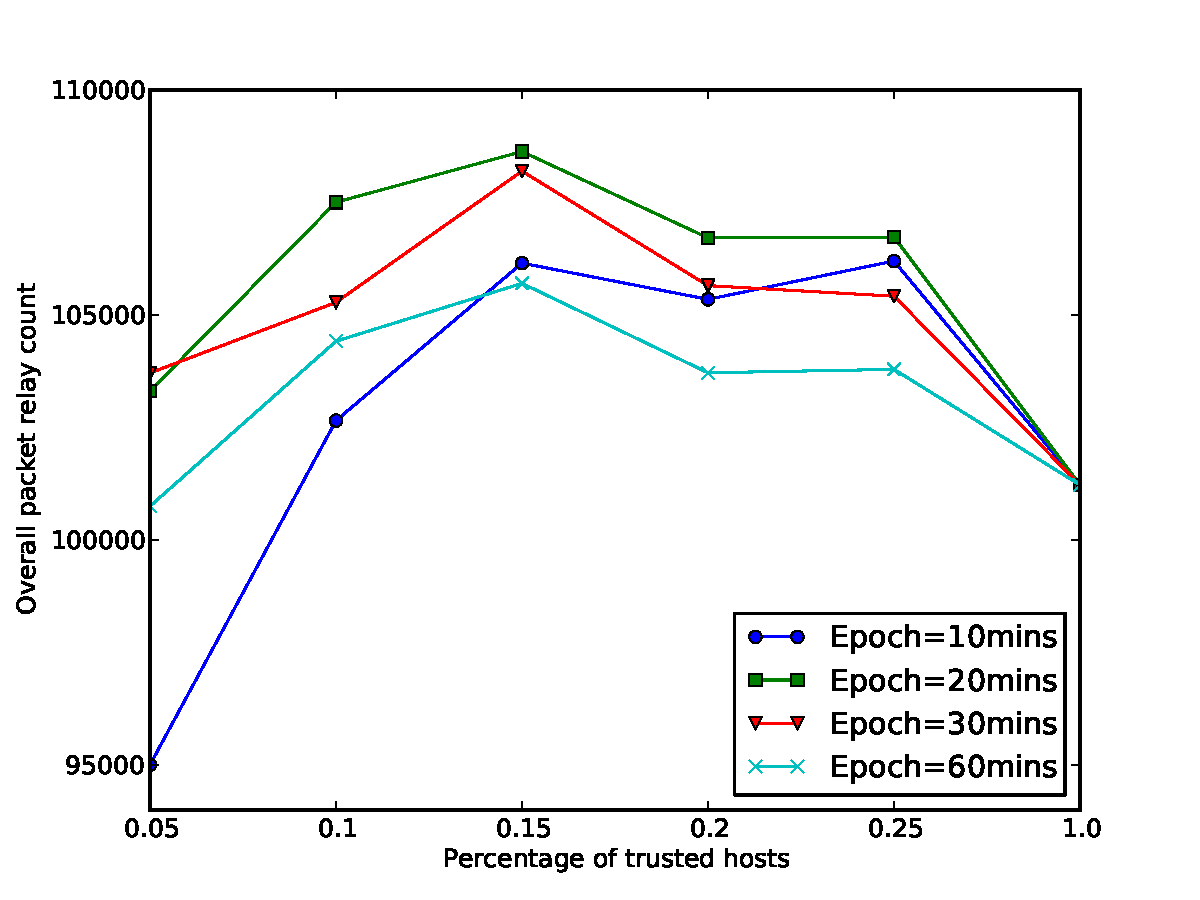
\includegraphics[width=0.49\columnwidth]{figures/epoch_3/relay_count.pdf}
\label{fig:relay_count_epoch_3}
}
\hfill
\subfloat[Relay count of overall packets. Ephemeral ID valid for 6 epochs.]{%
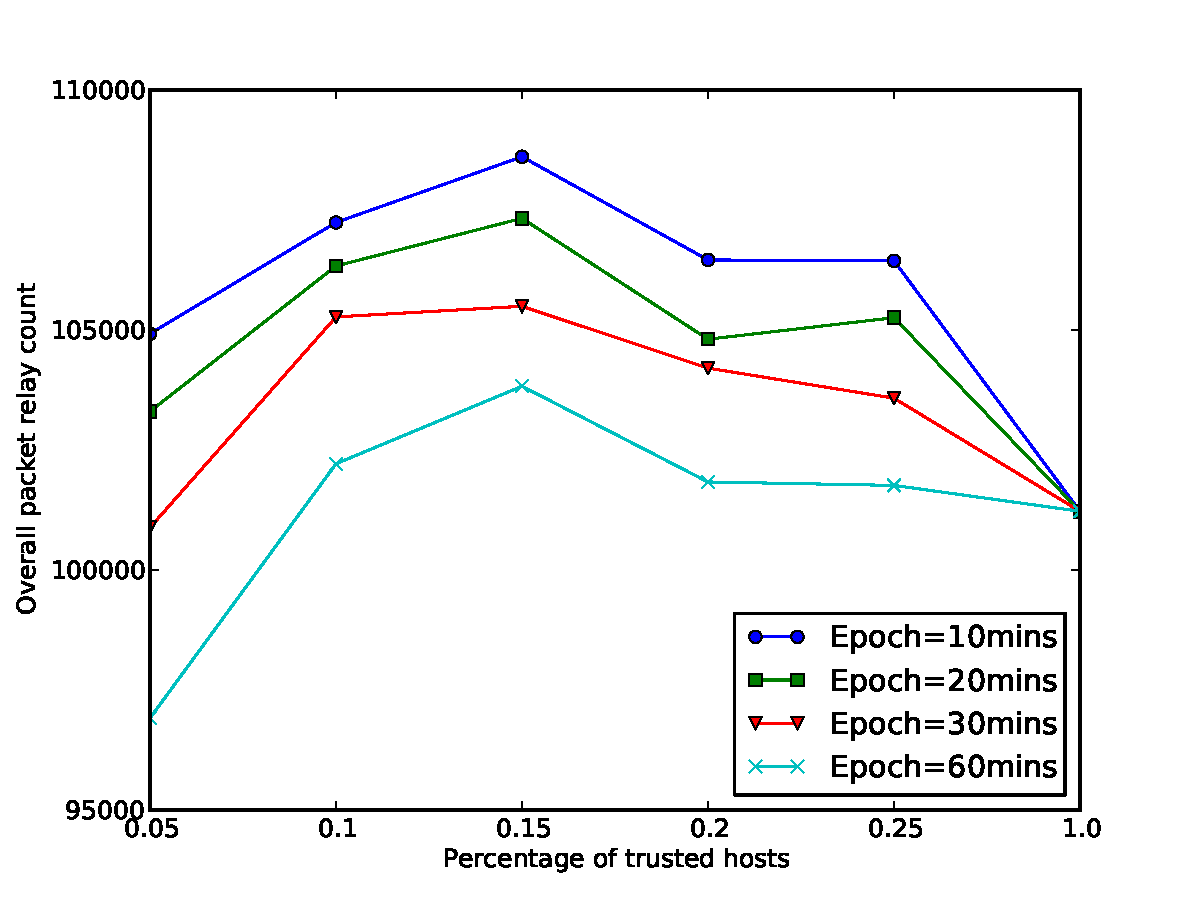
\includegraphics[width=0.49\columnwidth]{figures/epoch_6/relay_count.pdf}
\label{fig:relay_count_epoch_6}
}
\hfill
\subfloat[Relay count of delivered packets only. Ephemeral ID valid for 3 epochs.]{%
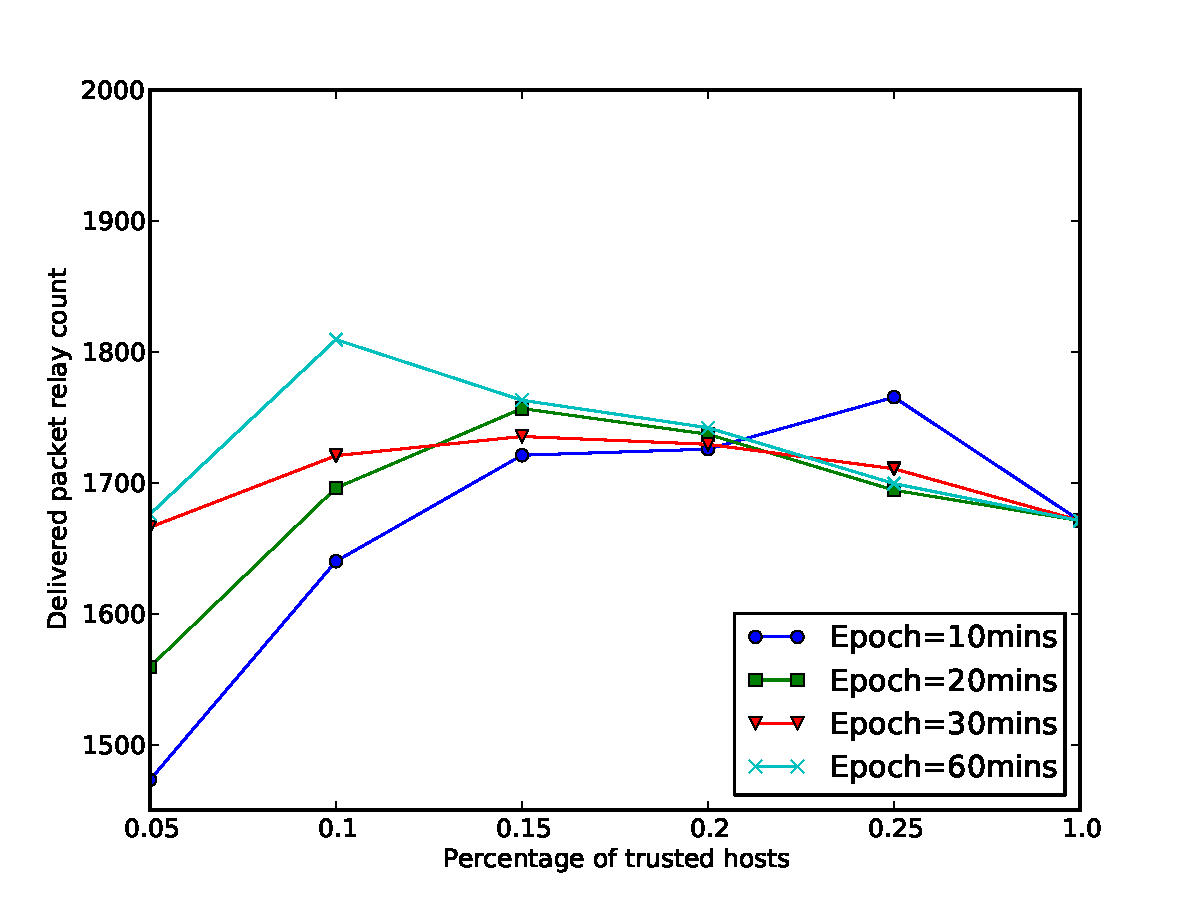
\includegraphics[width=0.49\columnwidth]{figures/epoch_3/relay_delivery_count.pdf}
\label{fig:relay_delivery_count_epoch_3}
}
\hfill
\subfloat[Relay count of delivered packets only. Ephemeral ID valid for 6 epochs.]{%
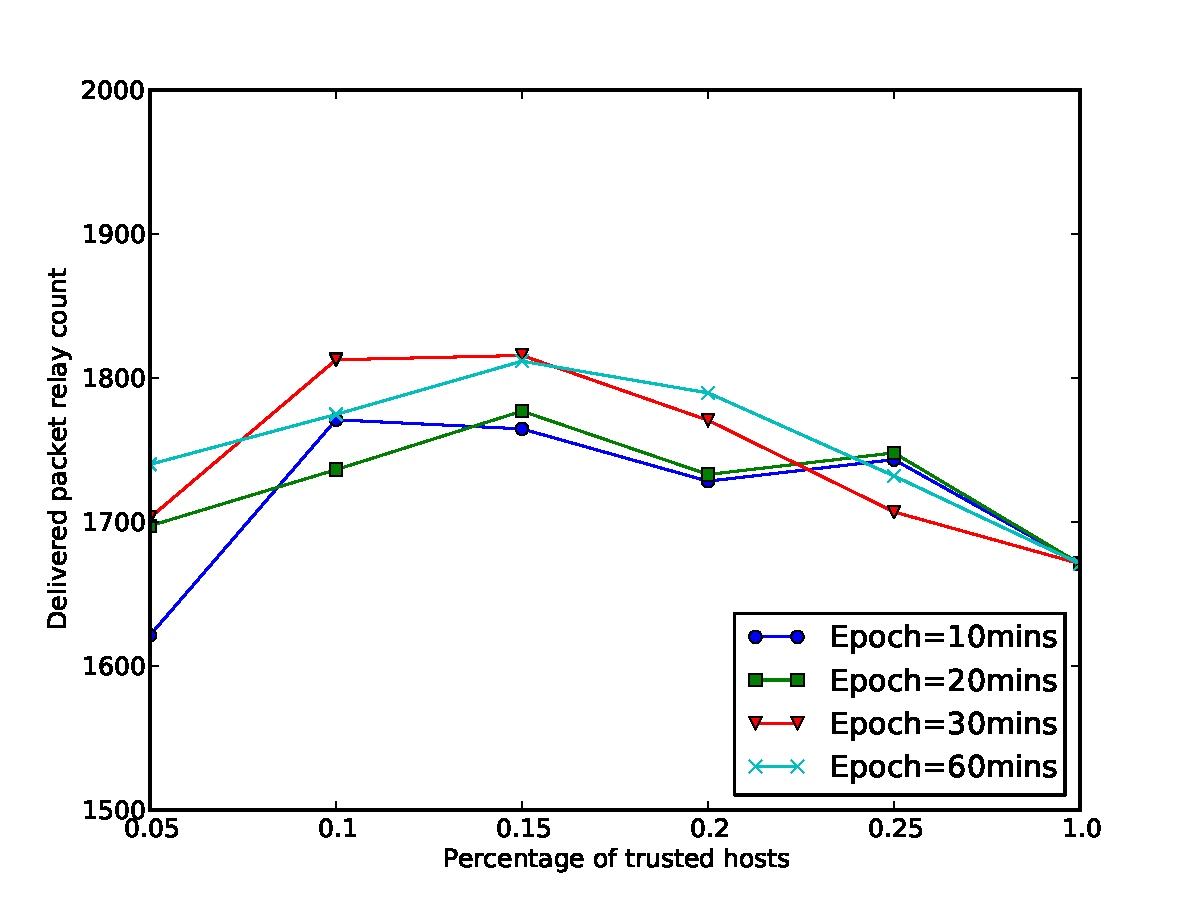
\includegraphics[width=0.49\columnwidth]{figures/epoch_6/relay_delivery_count.pdf}
\label{fig:relay_delivery_count_epoch_6}
}

\caption{{\bf Packet relay count.}
In flood-based routing protocol, only about $5\%$ of packet relays are used for actual packet deliveries. 
When the percentage of trusted nodes is less than $10\%$, the number of relays for delivered packets is extremely low.
}
\label{fig:relay_count}
\end{figure}







% packet relay classification over varying eppoch
\begin{figure}[h!]
\center
\subfloat[Overall packet relay classification. Ephemeral ID valid for 3 epochs]{%
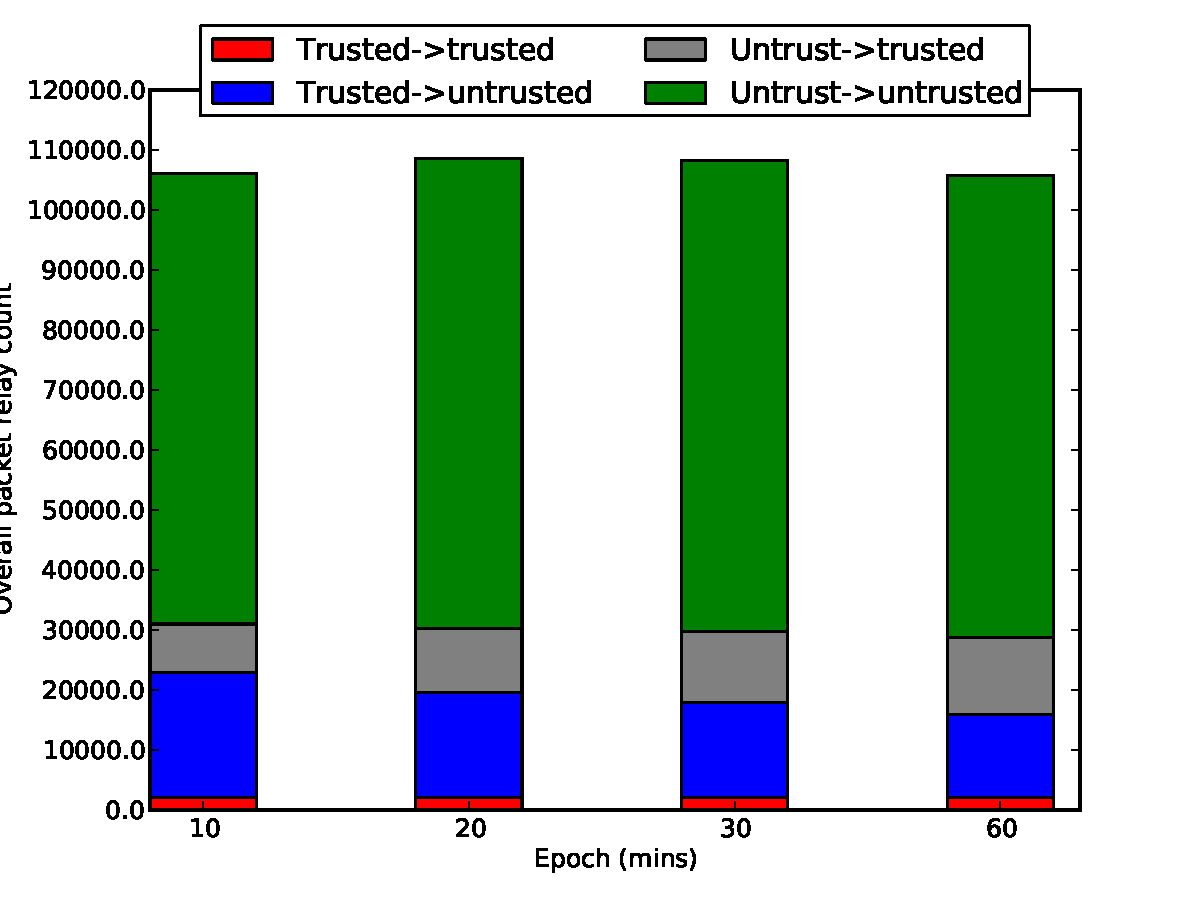
\includegraphics[width=0.49\columnwidth]{figures/epoch_3/relay_classification_over_epoch.pdf}
\label{fig:overall_relay_classification_epoch_3}
}
\hfill
\subfloat[Overall packet relay classification. Ephemeral ID valid for 6 epochs]{%
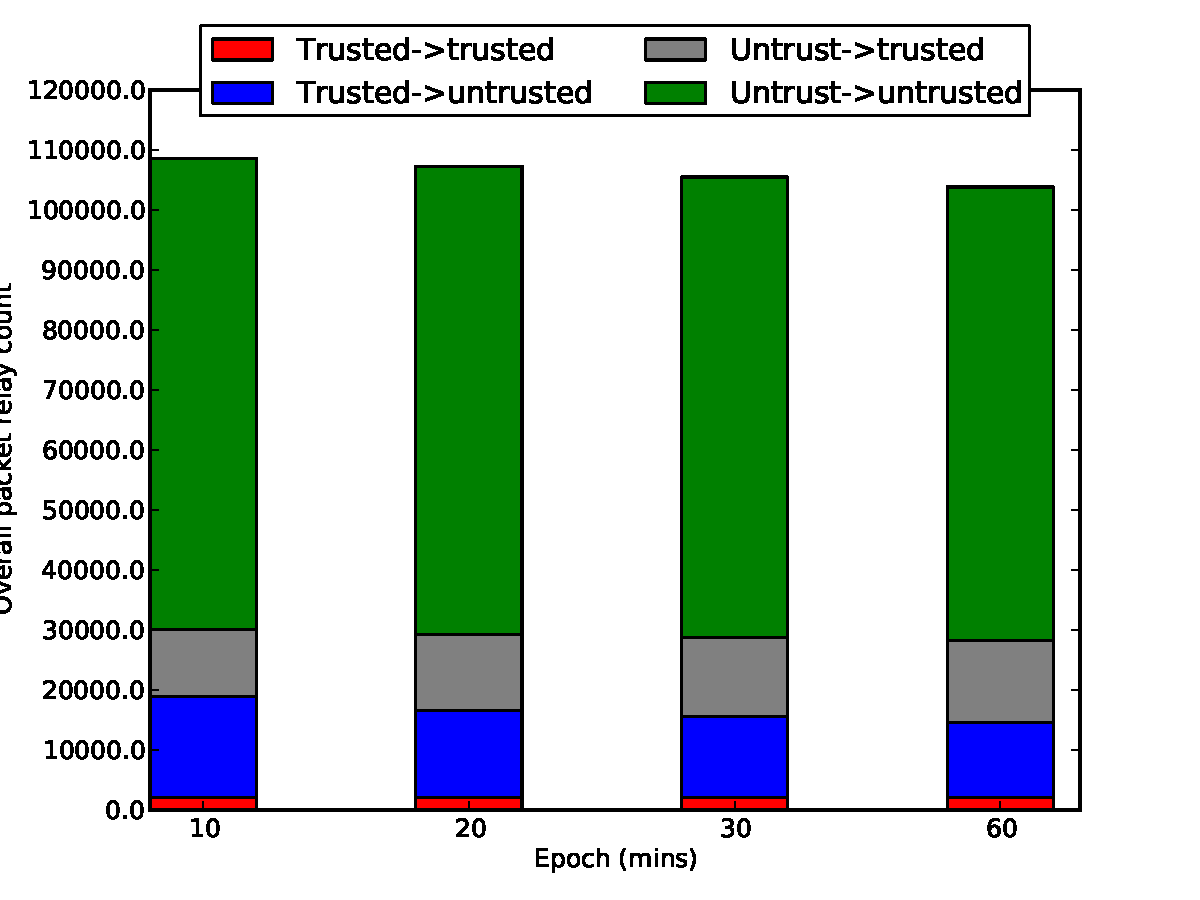
\includegraphics[width=0.49\columnwidth]{figures/epoch_6/relay_classification_over_epoch.pdf}
\label{fig:overall_relay_classification_epoch_6}
}
\hfill
\subfloat[Delivered packet relay classification. Ephemeral ID valid for 3 epochs]{%
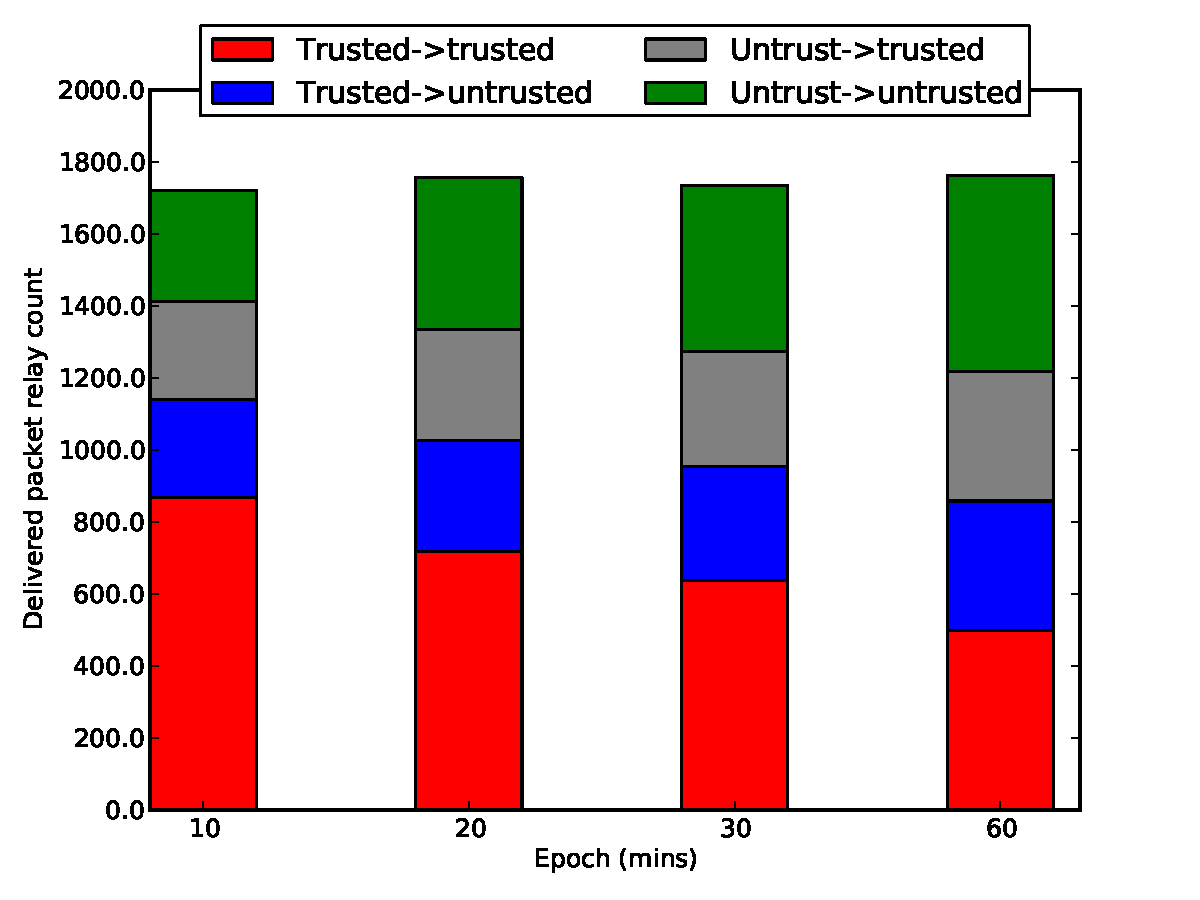
\includegraphics[width=0.49\columnwidth]{figures/epoch_3/relay_delivery_classification_over_epoch.pdf}
\label{fig:delivered_relay_classification_epoch_3}
}
\hfill
\subfloat[Delivered packet relay classification. Ephemeral ID valid for 6 epochs]{%
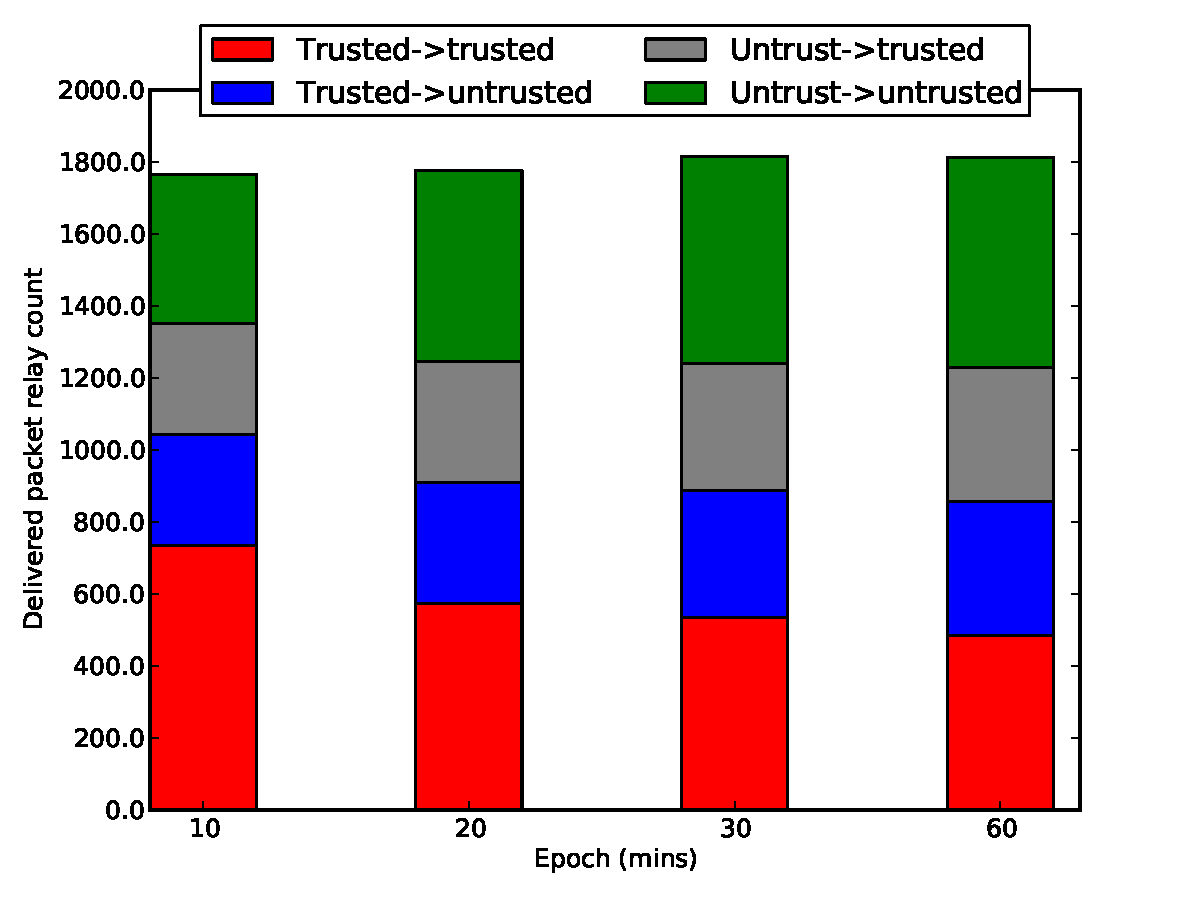
\includegraphics[width=0.49\columnwidth]{figures/epoch_6/relay_delivery_classification_over_epoch.pdf}
\label{fig:delivered_relay_classification_epoch_6}
}

\caption{{\bf Packet relay classification over varying epoch. Percentage of trusted nodes is $20\%$.}
Relay classification is not significantly different across different epochs. 
}
\label{fig:relay_classification_epoch}
\end{figure}




% packet relay classification over varying percentage of trusted nodes
\begin{figure}[h!]
\center
\subfloat[Overall packet relay classification. Ephemeral ID valid for 3 epochs.]{%
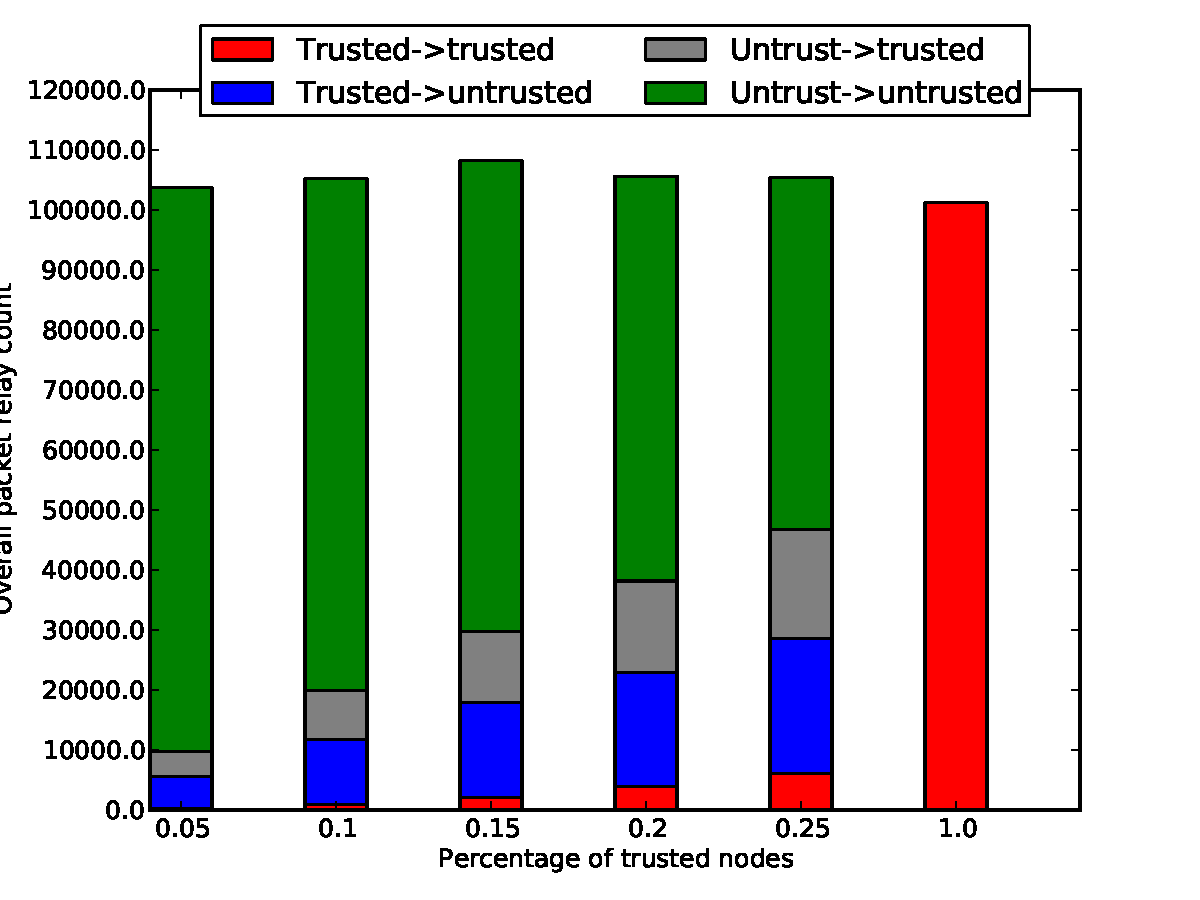
\includegraphics[width=0.49\columnwidth]{figures/epoch_3/relay_classification_over_percentage.pdf}
\label{fig:relay_classification_percentage_3}
}
\hfill
\subfloat[Overall packet relay classification. Ephemeral ID valid for 6 epochs.]{%
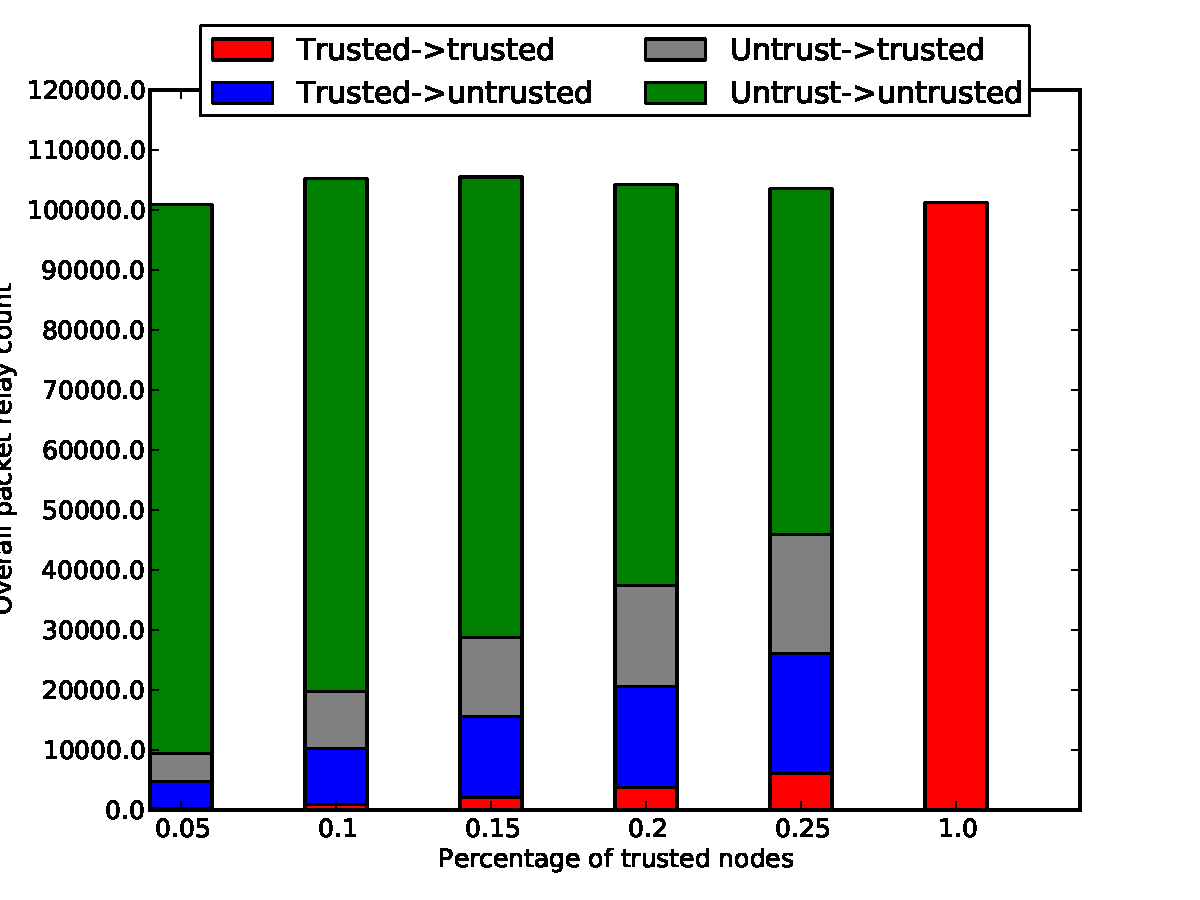
\includegraphics[width=0.49\columnwidth]{figures/epoch_6/relay_classification_over_percentage.pdf}
\label{fig:relay_classification_percentage_6}
}

\hfill
\subfloat[Delivered packet relay classification. Ephemeral ID valid for 3 epochs.]{%
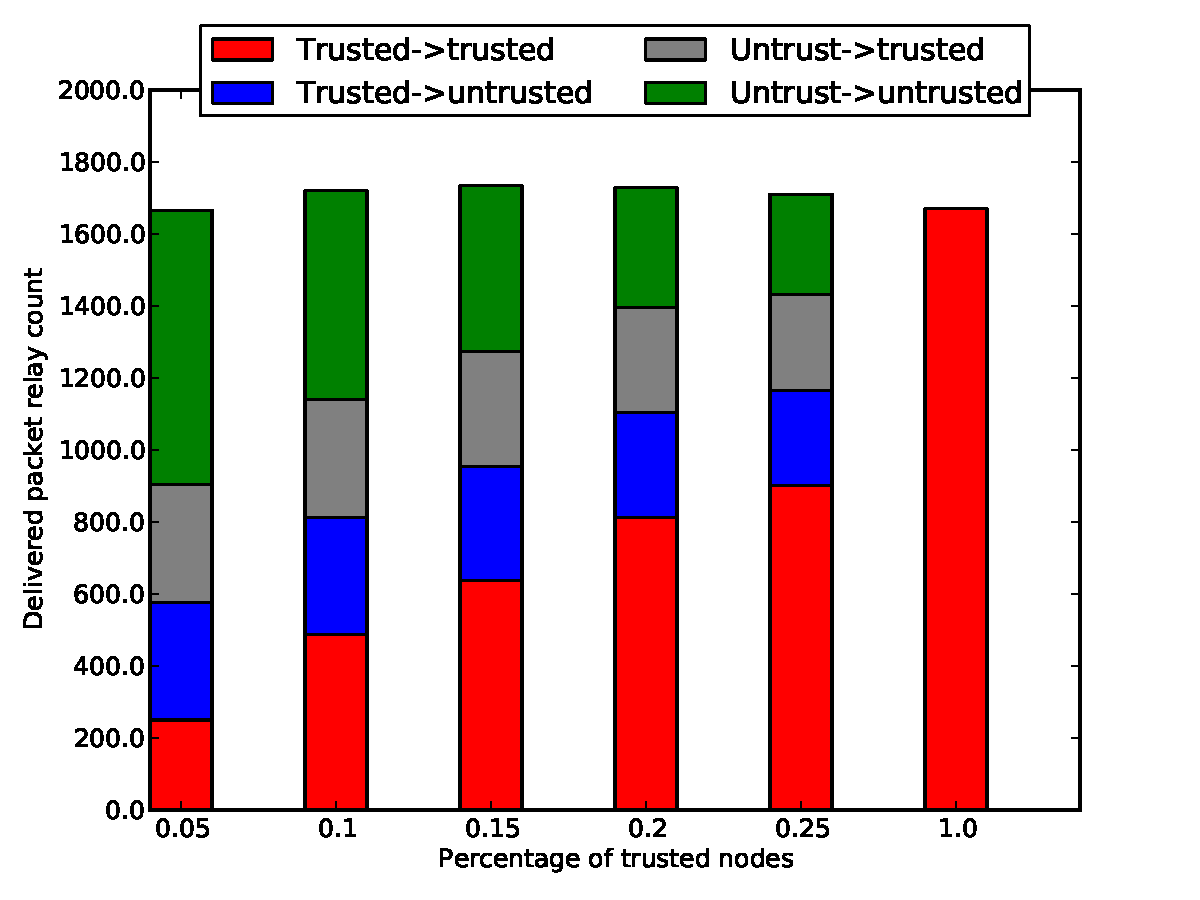
\includegraphics[width=0.49\columnwidth]{figures/epoch_3/relay_delivery_classification_over_percentage.pdf}
\label{fig:delivered_relay_classification_percentage_3}
}
\hfill
\subfloat[Delivered packet relay classification. Ephemeral ID valid for 6 epochs.]{%{%
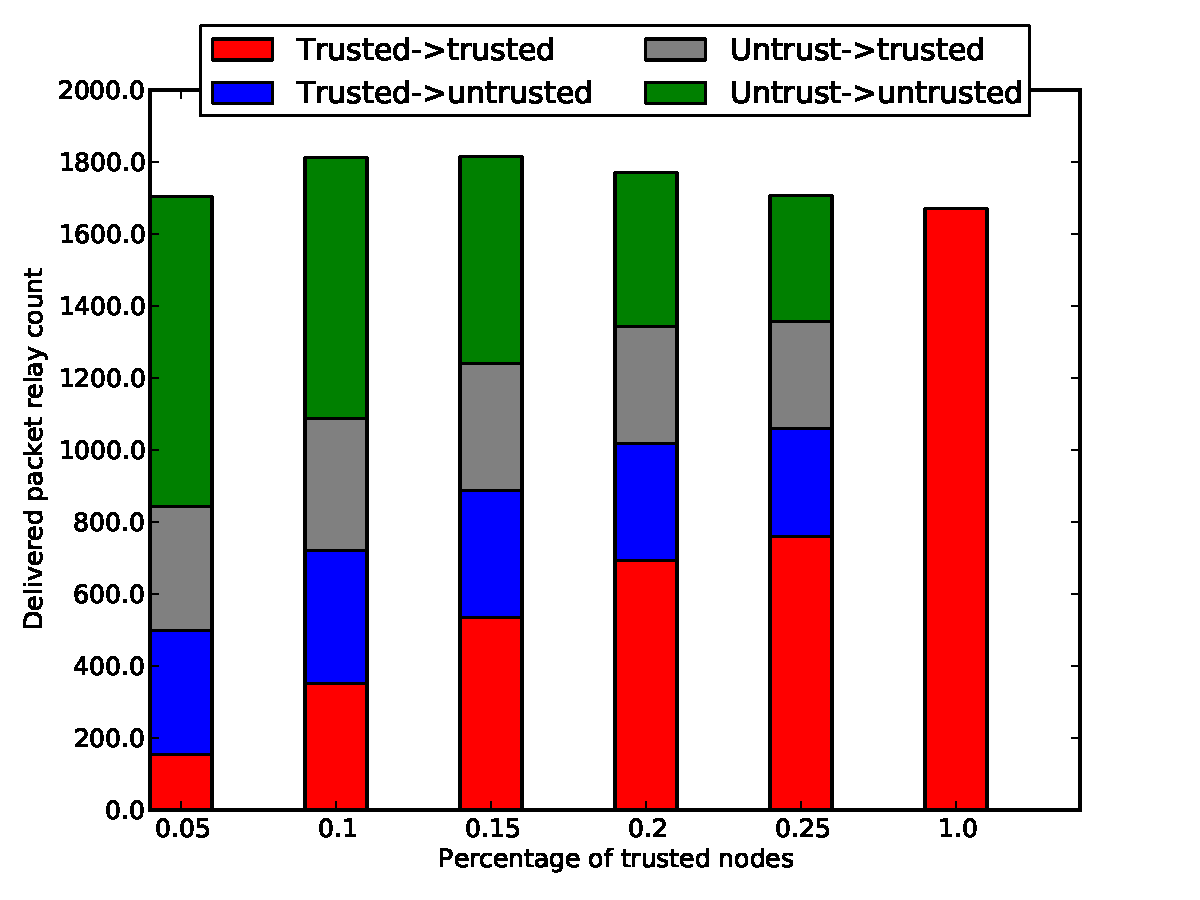
\includegraphics[width=0.49\columnwidth]{figures/epoch_6/relay_delivery_classification_over_percentage.pdf}
\label{fig:delivered_relay_classification_percentage_6}
}

\caption{{\bf Packet relay classification over varying percentage of trusted nodes. Epoch is $30$ mins.}
As in Figure~\ref{fig:relay_classification_epoch}, relays between two untrusted nodes account for relatively small part while relays between two trusted nodes account for the largest part (in most cases) in delivered packet relay classification. 
}
\label{fig:relay_classification_percentage}
\end{figure}




% packet drop classification
\begin{figure}[h!]
\center
\subfloat[Packet drops over varied epoch. Percentage of trusted nodes = 0.2. Ephemeral ID valid for 3 epochs.]{%
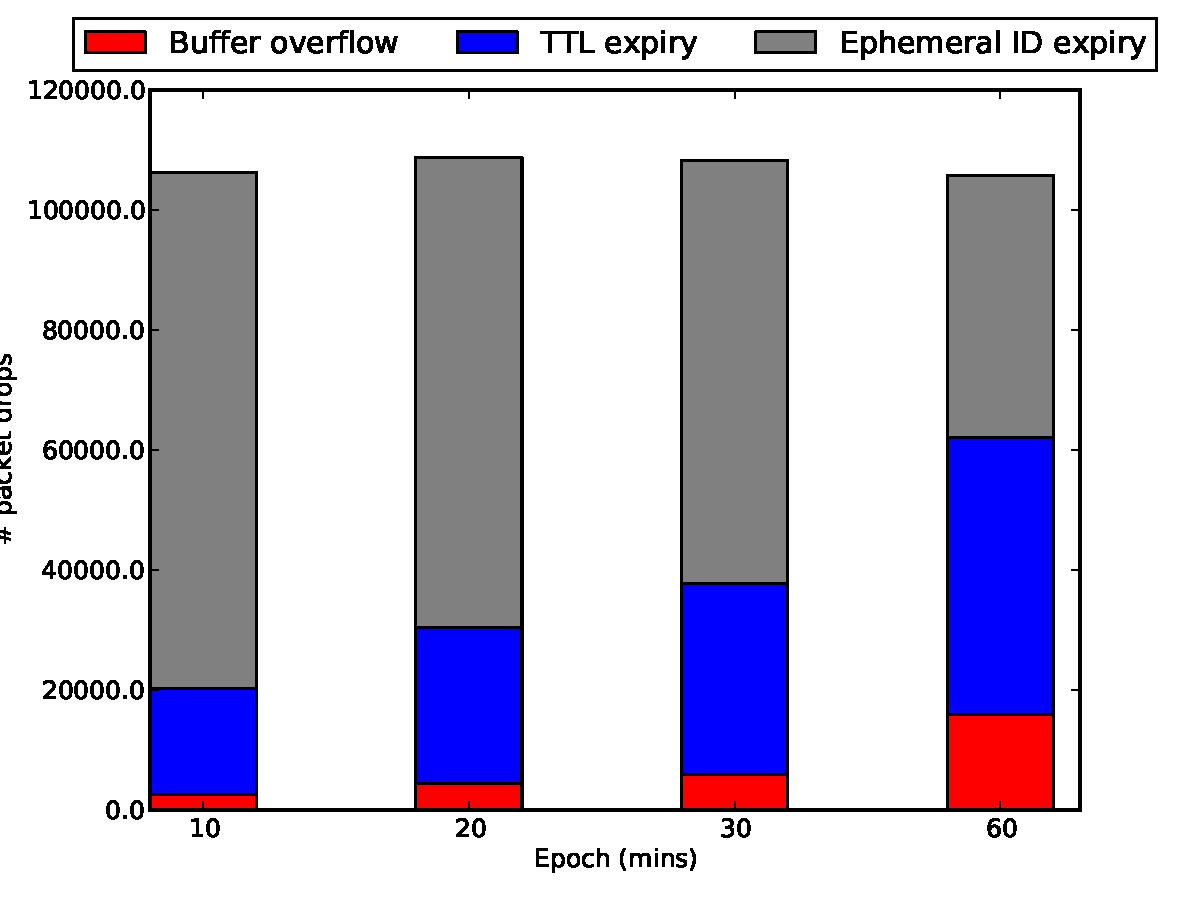
\includegraphics[width=0.49\columnwidth]{figures/epoch_3/drop_classification_over_epoch.pdf}
\label{fig:drop_classification_epoch_3}
}
\hfill
\subfloat[Packet drops over varied epoch. Percentage of trusted nodes = 0.2. Ephemeral ID valid for 6 epochs.]{%
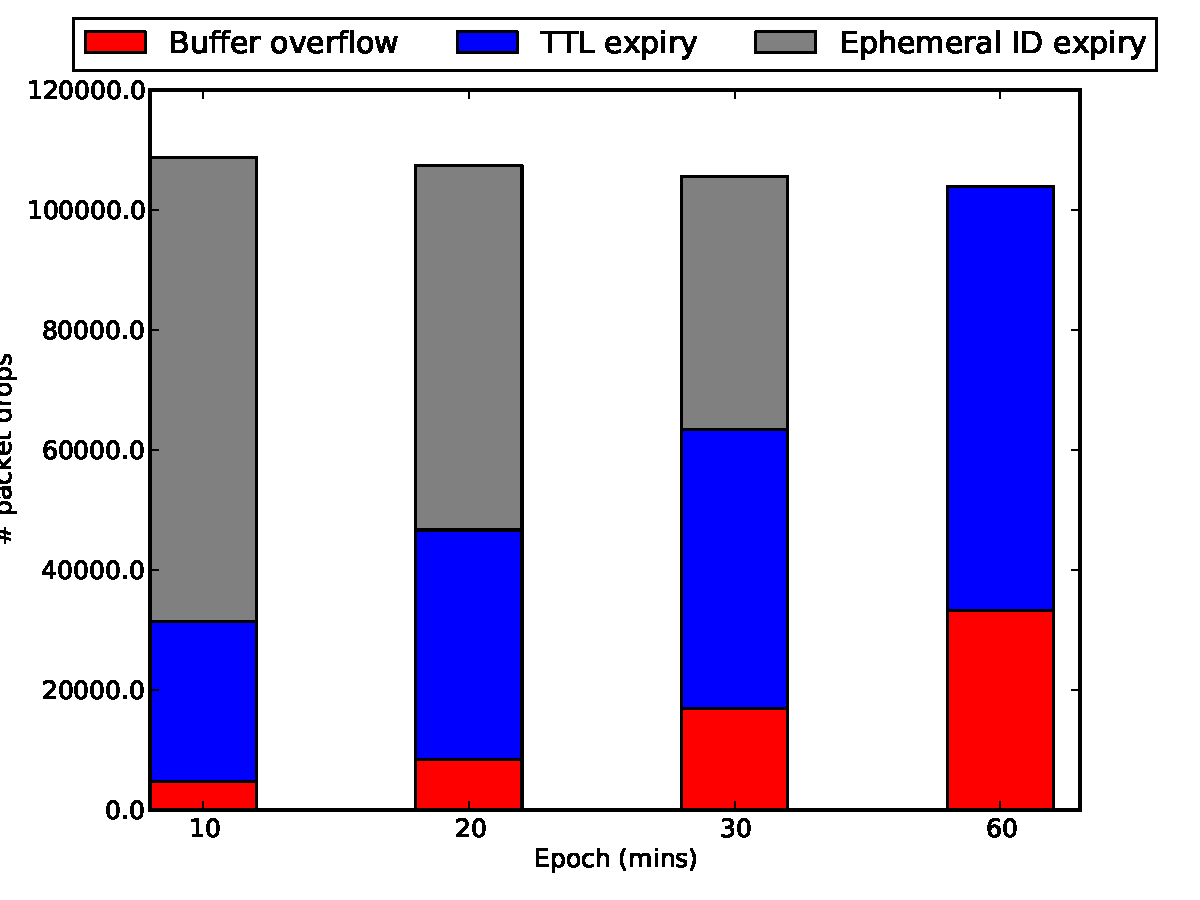
\includegraphics[width=0.49\columnwidth]{figures/epoch_6/drop_classification_over_epoch.pdf}
\label{fig:drop_classification_epoch_6}
}
\hfill
\subfloat[Packet drops over varied percentage of trusted nodes. Epoch = 30 mins. Ephemeral ID valid for 3 epochs.]{%
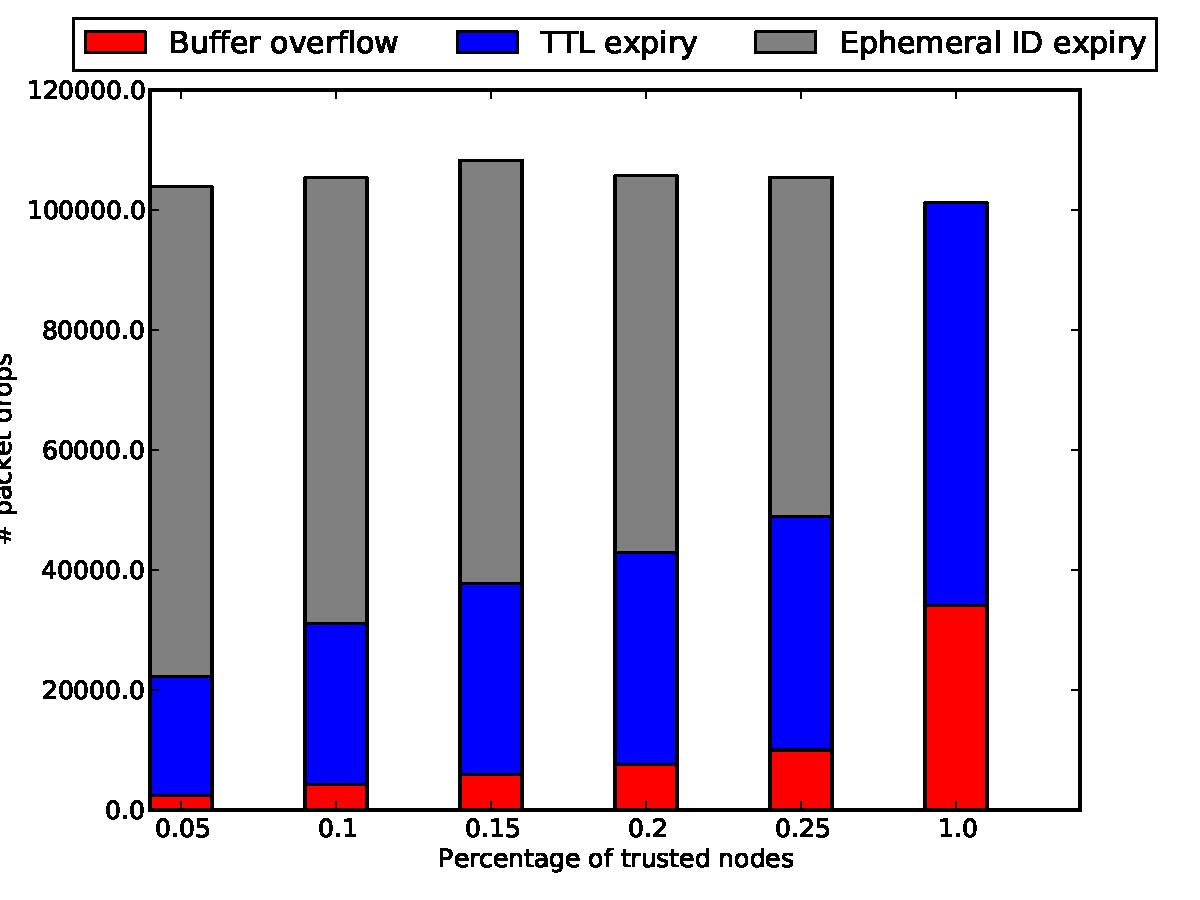
\includegraphics[width=0.49\columnwidth]{figures/epoch_3/drop_classification_over_percentage.pdf}
\label{fig:drop_classification_percentage_3}
}
\subfloat[Packet drops over varied percentage of trusted nodes. Epoch = 30 mins. Ephemeral ID valid for 6 epochs.]{%
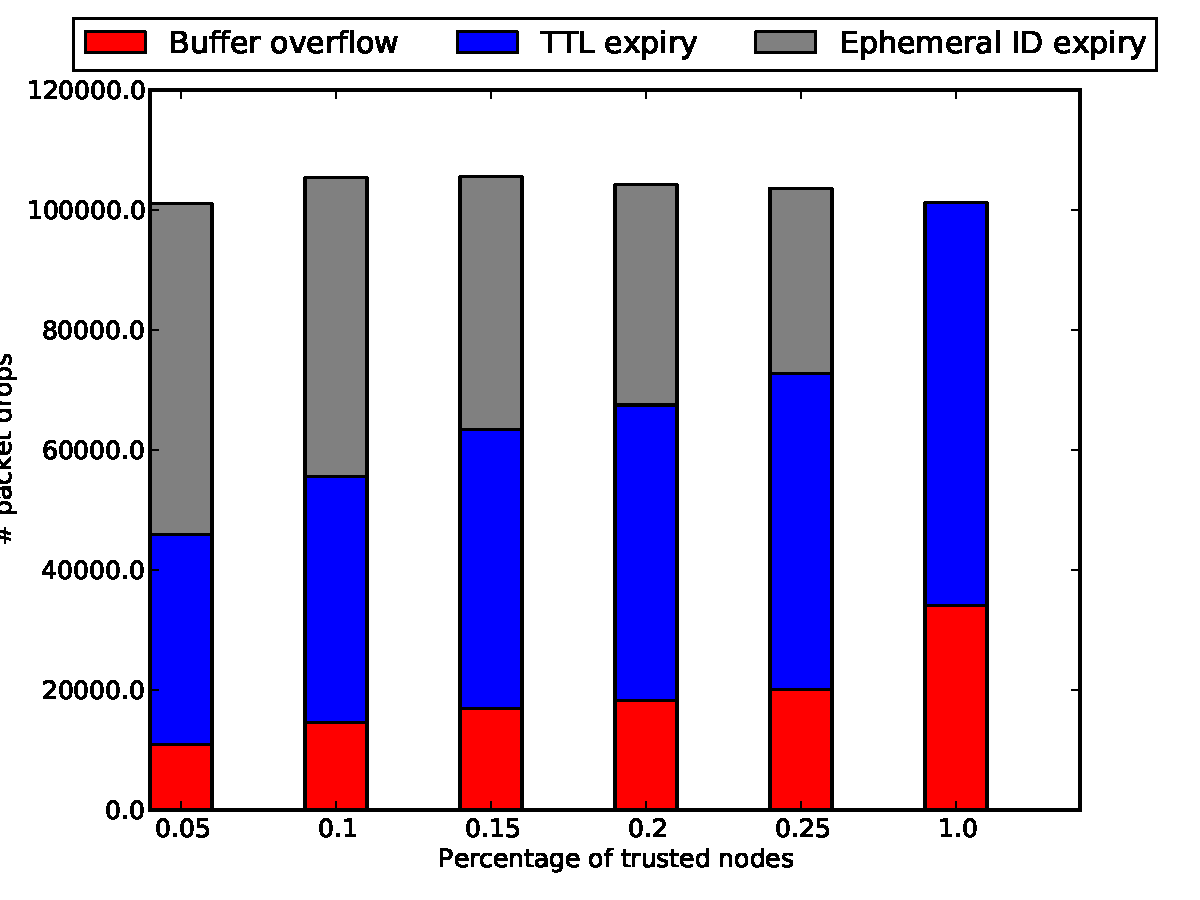
\includegraphics[width=0.49\columnwidth]{figures/epoch_6/drop_classification_over_percentage.pdf}
\label{fig:drop_classification_percentage_6}
}
\caption{{\bf Packet drop classification.}
With ephemeral ID valid for 6 epochs (Figures~\ref{fig:drop_classification_epoch_6} and \ref{fig:drop_classification_percentage_6}),  
the total number of packet drops is slightly decreased compared to when ephemeral ID valid for 3 epochs is used (Figures~\ref{fig:drop_classification_epoch_3} and \ref{fig:drop_classification_percentage_3}), mainly because packet drops due to ephemeral ID expiry is decreased.
}
\label{fig:drop_classification}
\end{figure}






% packet delivery count with untrusted nodes
\begin{figure}[t!]
\center
\subfloat[Packet deliveries with untrusted nodes: Ephemeral ID valid for 3 epochs.]{%
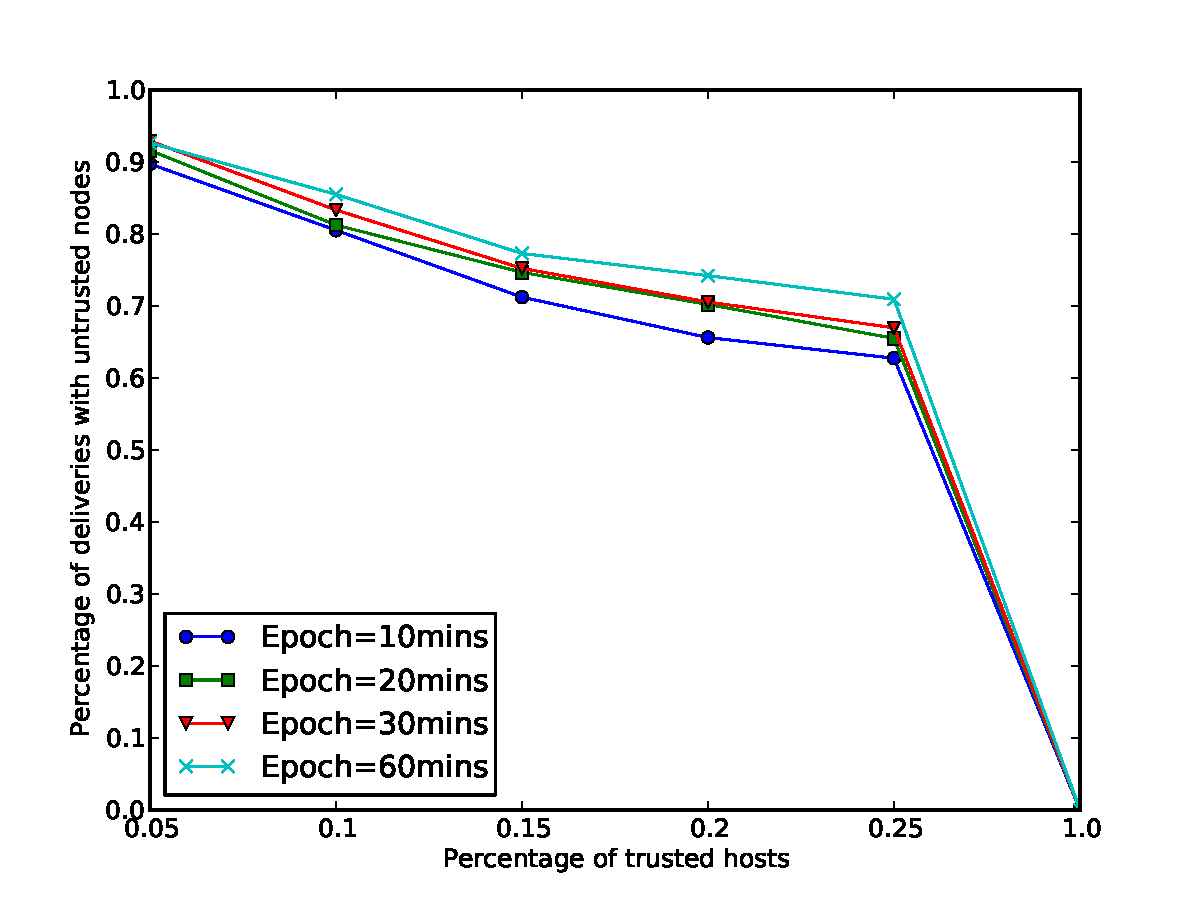
\includegraphics[width=0.49\columnwidth]{figures/epoch_3/delivery_with_ut.pdf}
\label{fig:delivery_ut_3}
}
\hfill
\subfloat[Packet deliveries with untrusted nodes: Ephemeral ID valid for 6 epochs.]{%
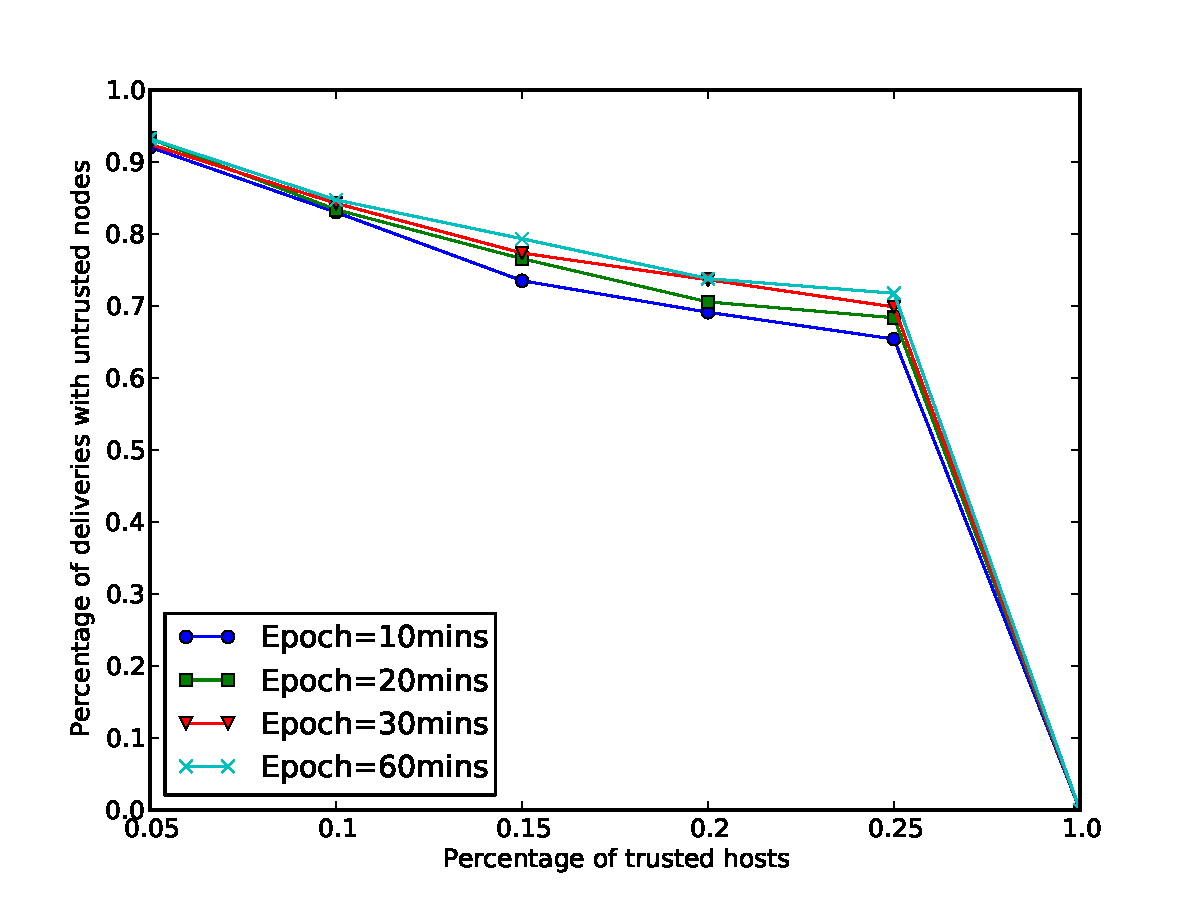
\includegraphics[width=0.49\columnwidth]{figures/epoch_6/delivery_with_ut.pdf}
\label{fig:delivery_ut_6}
}
\caption{{\bf Packet deliveries with untrusted nodes.}}
\label{fig:delivery_count}
\end{figure}




% average relay count per message
\begin{comment}
\begin{figure}[h!]
\center
\subfloat[Average relay count per message. Ephemeral ID valid for 1 epoch]{%
\includegraphics[width=0.49\columnwidth]{figures/epoch_3/relay_per_message.pdf}
\label{fig:relay_per_message_3}
}
\hfill
\subfloat[Average relay count per message. Ephemeral ID valid for 3 epochs]{%
\includegraphics[width=0.49\columnwidth]{figures/epoch_6/relay_per_message.pdf}
\label{fig:relay_per_message_6}
}
\caption{{\bf Average relay counts per message.}
With ephemeral ID valid for 1 epoch, packets are not relayed enough times since the packets are dropped mainly due to ephemeral ID expiry, especially when the percentage of trusted node is low (Figure~\ref{fig:relay_per_message_3}). 
By using ephemeral ID valid for 3 epochs, the average relay count per message stays almost same regardless of the percentage of trusted nodes.
}
\label{fig:relay_per_message}
\end{figure}
\end{comment}



\end{document}







